\documentclass[11pt,letterpaper]{article}

\usepackage{natbib}
%\usepackage{cite}
\usepackage{graphicx}
\usepackage[margin=1.in,centering]{geometry}
\usepackage{hyperref}
\usepackage{caption}
\usepackage[export]{adjustbox}
\usepackage{float}

\begin{document}

\title{Computational Anomalies in Error Estimation}
\date{August 25, 2016}

Dear Dr. Cackett,\\


Here are some musings on the computational anomalies seen in the results of the psdlag program. I cover some things about the input script, some calculations that didn't converge, and the error modes and results. I did my best to create grids of the error results, but compiling a grid from the error mode "1" results produces some pretty whacky results, and this is probably a problem with my graphing routines not working properly without a complete set of analyses -- that is, psdlag output files.

\section{Input Script}
I've included a psdlag input script which is made from the template I use, but each wavelength has its own initial parameters extracted from the err0 results. In the template, I use 0:0 0 to designate the basis light curve; however, this does differ from the original document you gave to me at the beginning of the summer. I don't remember the specifics of why I changed from the original to this form, but I came to that conclusion after some explorations and discussion with you. I'm confident I could reconstruct that, but perhaps this is where a mistake was made. This script and the files needs to run it are included in the .tar.gz file.

Example input script: \\
2\\
1367A.lc 0\\
1479A.lc 0\\
8 0.0049999999 0.018619375 0.044733049 0.069336227 0.10747115 0.16658029 0.25819945 0.40020915 0.62032418\\
0\\
6.533e-02 -9.694e-02 -1.175e+00 -1.525e+00 -2.166e+00 -2.492e+00 -3.258e+00 -9.328e+00 0.2e+00 -0.2e+00 -1.0e+00 -1.500e+00 -2.0e+00 -2.6e+00 -3.4e+00 -6e+00 9.340e-02 -8.842e-02 -1.173e+00 -1.512e+00 -2.113e+00 -2.547e+00 -3.178e+00 -7.000e+00 -6.035e-02 2.044e-02 1.258e-01 5.764e-02 2.580e-02 -4.737e-02 9.579e-02 6.411e-01\\
0:0 0\\
2\\
0\\
1000 50 400 mcmc\_1479A.dat\\

\section{Outputs of Each Error Mode}
I'll print grids of results for each error type. I will also include the psdlag output files for each analysis. It will be important for me to explain the filename format if you want to read the correct files. The first number in the filename is the wavelength of the reference band, which is succeeded by the wavelength of the reverberated band. In brackets, the timestep is given (should be 0.01 days) and finally the error type: $\sigma \in CM/LF/MC$. This allows one to know which error mode was used when running psdlag to produce the output.

Psdlag includes three methods for computing errors, or error modes. These are designated by an integer from 0-2:\\
- 0: Extracting from the covariance matrix (CM)\\
- 1: Scanning the likelihood function (LF) \\
- 2: Monte Carlo (MC)\\

\subsection{Error Mode 0 - Covariance Matrix (CM)}
The covariance matrix method, i.e. the "quick" method, is the method we had our early successes with. Here are the grids of PSD and timelags. We do see some possible issues with errors here, with those that are too small and one that is extremely large. Very small errors may be expected here since this method doesn't account for error dependencies across bins. I'm not sure what's going on with the very large errors in the 3465\AA$ $ time lags;  the solution to the cross spectrum converges very quickly: within 11 steps, compared to often closer to 100 or 150 steps. It may need some different initial parameters, so I'll try that, but the convergence can be seen starting at a somewhat lower value (371), with a nice grade toward the likelihood value of 430, so I'm not terribly hopeful. These are both higher than the typical output: usually the program stops solving as the likelihood settles to 300-350.

\begin{figure}
    \label{fig:psd_err0}
    \centering
    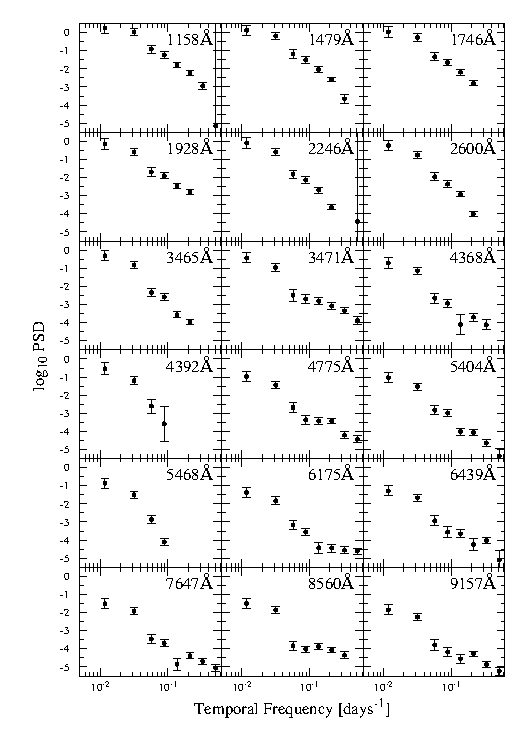
\includegraphics{../img/psd_atlas_err0.pdf}
    \caption{PSD from psdlag using error mode 0 (CM).}
\end{figure}

\begin{figure}
    \label{fig:lag_err0}
    \centering
    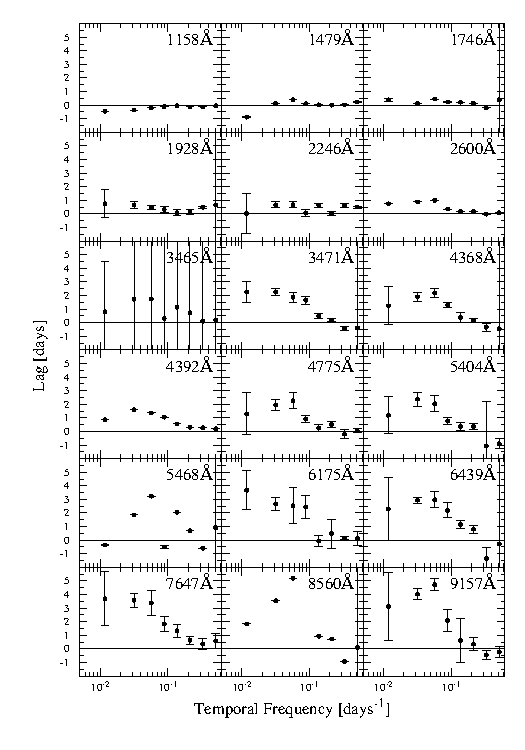
\includegraphics{../img/timelag_atlas_err0.pdf}
    \caption{Time lag for psdlag run using error mode 0 (CM). These are the results included in my final report. }
\end{figure}

\subsection{Error Mode 1 - Scanning Likelihood Function (LF)}
This is probably the preferred way of computing the variance of the PSD and time lags. Many of analyses in this group did not finish due to either the convergence routine not starting or not stepping the parameters. For example, in 1928\AA, under parameter 1 (the second parameter), the output shows:\\

******* par 1 *******\\
1 7.01525e-05 36.107 0.0736126 -0.197534 -1.18167 -1.52074 -2.14419 -2.50319 -3.58007 -12.328 \\
1 7.01525e-05 36.107 0.0736126 -0.197534 -1.18167 -1.52074 -2.14419 -2.50319 -3.58007 -12.328 \\
1 7.01525e-05 36.107 0.0736126 -0.197534 -1.18167 -1.52074 -2.14419 -2.50319 -3.58007 -12.328 \\

and these lines are repeated ad infinitum, so there is clearly no convergence happening here. I have attempted other initial parameters. The following analyses showed such a situation:\\
    - 1746\AA\\
    - 1928\AA\\
    - 2246\AA\\
    - 2600\AA\\
    - 3465\AA\\
    - 4368\AA\\

The analyses that did not finish because the optimization routine didn't start show as a last line in the output file something like:\\
******* par 7 *******\\

with no succeeding lines. This includes:\\
- 1497\AA\\
- 4382\AA\\
- 5468\AA\\
- 8560\AA\\

When I learned that these optimizations were not working, I stopped the other models, so some models did not finish. I then moved on to the Monte Carlo method.

\begin{figure}
    \label{fig:psd_err1}
    \centering
    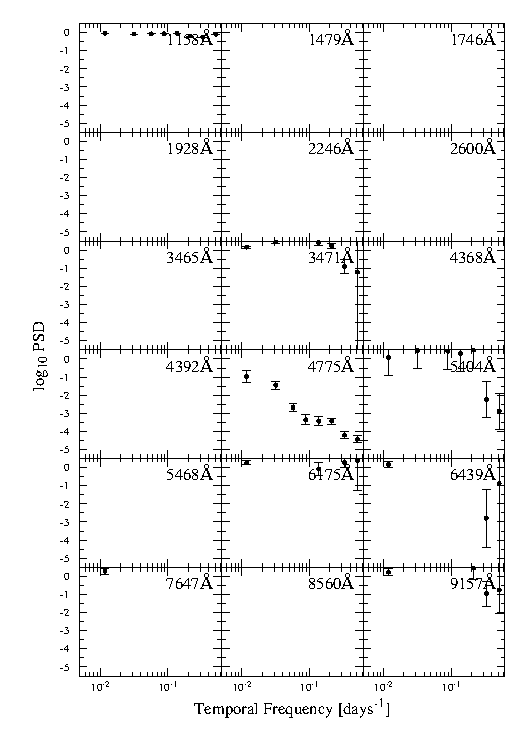
\includegraphics{../img/psd_atlas_err1.pdf}
    \caption{PSD from psdlag using error mode 1 (LF). Most of these models did not finish, so the grid is very sparse and may be misreporting values due to a lack of proper scraping logic.}
\end{figure}

\begin{figure}
    \label{fig:lag_err1}
    \centering
    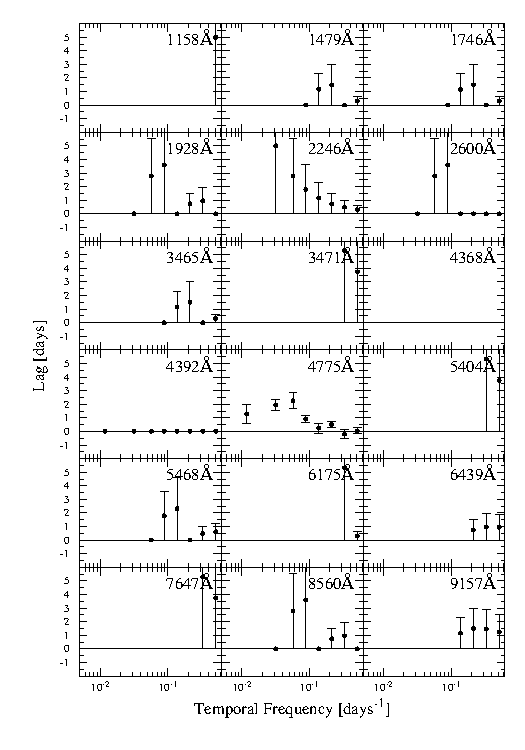
\includegraphics{../img/timelag_atlas_err1.pdf}
    \caption{Time lag for psdlag run using error mode 1 (LF). Most of these models did not finish, so the grid is very sparse and may be misreporting values due to a lack of proper scraping logic.}
\end{figure}



\subsection{Error Mode 2 - Monte Carlo (MC)}
This is the method we ultimately tried to get working for my final presentation, but were unsuccessful. Chia-ying told me that she has used this method for analyses in the past, and chose to do so because she was unable to get LF to work. 4392\AA$ $ and 5404\AA$ $ did not finish, so they're meaningless: that means they took over 48 hours to run on a computation node on our cluster at WMU. That might indicate a problem unto itself. 1756\AA$ $ did finish, with those results. Ultimately, we decided that the errors on the timelags didn't make much sense, which is why I never went back to complete the remaining two models.

I tried to look through the output files for clues, but in the end, I could find no apparently pattern indicated why any models showed strange results, with either strong or weak variance. I may not be keen enough to notice the important values popping up in the optimization readouts in the output files, but I did notice that 1928\AA$ $ and 4368\AA$ $ oscillate to the final 400$^{th}$ step rather than converge. Many of these models take close to or more than 24 hours to run on cores at the WMU cluster, which are not top-of-the-line, but are reasonably modern and fast machines.


\begin{figure}
    \label{fig:psd_err2}
    \centering
    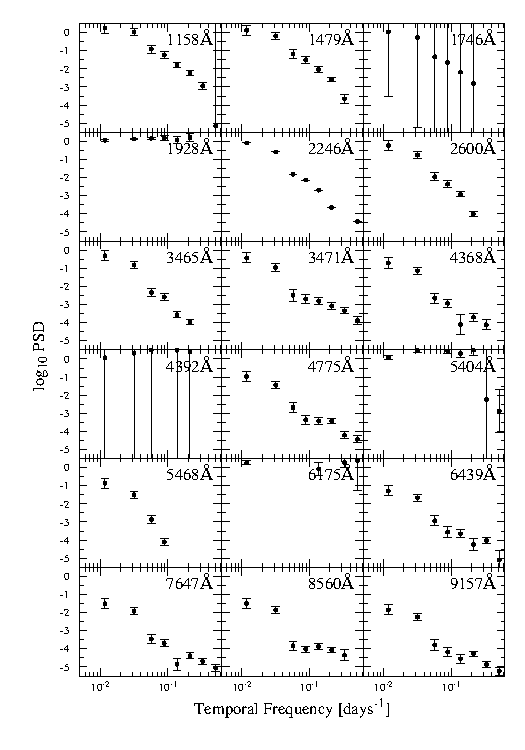
\includegraphics{../img/psd_atlas_err2.pdf}
    \caption{PSD from psdlag using error mode 2 (MC).}
\end{figure}


\begin{figure}
    \label{fig:lag_err2} 
    \centering
    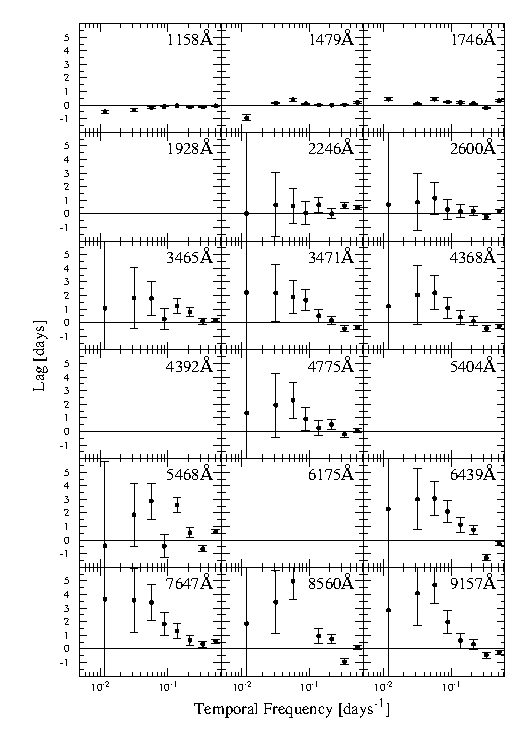
\includegraphics{../img/timelag_atlas_err2.pdf}
    \caption{Time lag for psdlag run using error mode 2 (MC).}
\end{figure}


\section{Closing}
That's all I have for now. I will keep changing things and trying new runs. I'll let you know if I find out anything new of importance. Hopefully some good can come from this.\\

Best Regards,

Otho Ulrich


\end{document}
